%# -*- coding:utf-8 -*-
\section{方法}
\label{sec7-2}

\subsection{Work Flow at A Glance}
\label{sec:overview}

Figure \ref{fig:DataFlow} illustrates the main steps taken in segmenting the heart from the CT information.
The raw data is firstly smoothed and is then thresholded into a well-shaped binary images.
Next, the preprocessed data is simultaneously distributed to compute the distance map and the edge potential map.
%Finally, the active contours are evolved toward the boundaries of the heart.
After that, the active contours are evolved toward the boundaries of the heart.
Finally, the resultant information is organized and rendered into a surface model.
\begin{figure}[t]
\centering
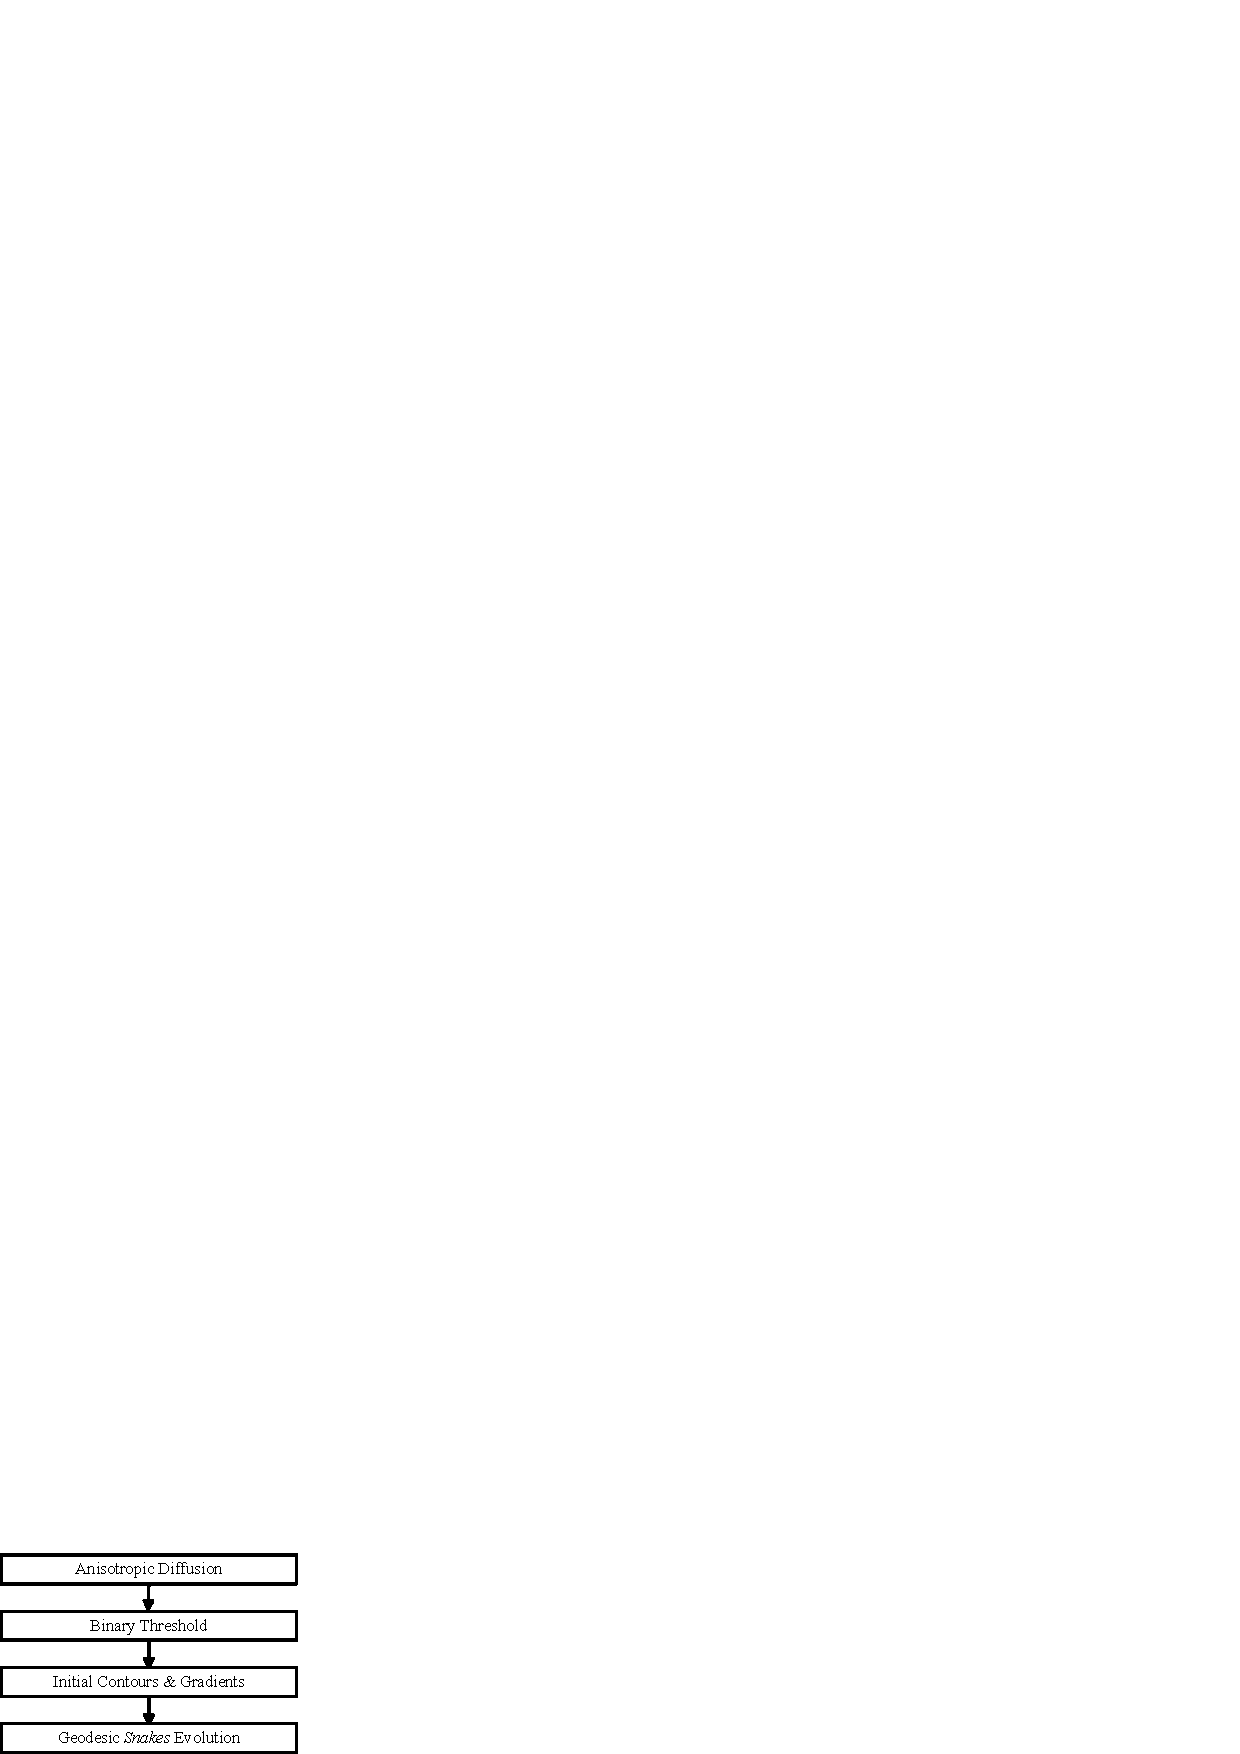
\includegraphics[height=2.0in]{Figures/chap07/DataFlow.pdf}
\caption{Flowchart of the segmentation work flow.}
\label{fig:DataFlow}
\end{figure}

\subsection{Preprocessing}
\label{sec:preprocessing}

\subsubsection{Smoothing with Edge Preservation}

The pepper noises introduced in the stage of image acquisition will considerably affect the following segmentation.
Thus the smoothing must be taken before any other processing steps.
The principle is to remove the noisy pixels as much as possible while to protect the details of the edge as complete as possible.
The smoothing algorithm based on the following \emph{modified curvature diffusion equation} (MCDE) \cite{Whitaker2001} is adopted:
\begin{equation}
\label{eqn:MCDE}
\frac{\partial I}{\partial t} = |\nabla I| \nabla \cdot c(|\nabla I|) \frac{\nabla I}{|\nabla I|},
\end{equation}
where $I(\cdot)$ represents the input image, $c$ is the conductance function given by $c(|\nabla I|) = k^2/(k^2 + |\nabla I|^2)$ with a free parameter $k$, determining the contrast of edges. %

\subsubsection{Binary Thresholding}

The thresholding is introduced to convert the images into the ``well-featured" ones, in which most of the uninterested contents will be excluded by assigning them a zero intensity value, while the contents of interest in a bright and uniform intensity (see Fig. \ref{fig:BinaryThresholdFunc}): %
\begin{equation}
\label{eqn:BinaryThreshold}
I_{\text{output}} =
\begin{cases}
255, & \text{lower} \le I_{\text{input}} \le \text{upper}, \\%
0,   & \text{otherwise}.
\end{cases}
\end{equation}
%\begin{figure}[t]
%\centering
%%# -*- coding:utf-8 -*-
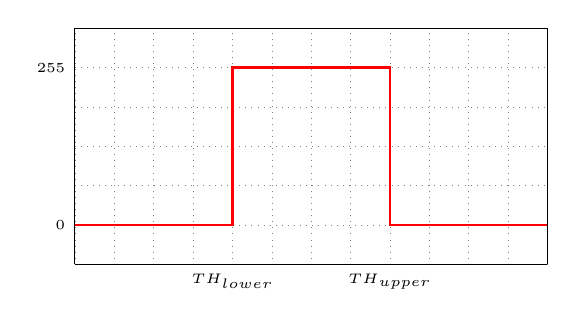
\begin{tikzpicture}[xscale=1.0,yscale=1.0]
\draw [help lines,dotted,step=.5] (0,0) grid (6,3);
\draw [thin] (0,0) -- (0,3);
\draw [thin] (0,3) -- (6,3);
\draw [thin] (0,0) -- (6,0);
\draw [thin] (6,0) -- (6,3);
\node [below] at (2,0) {\tiny$\text{TH}_{\text{lower}}$};
\node [below] at (4,0) {\tiny$\text{TH}_{\text{upper}}$};
\node [left] at (0,2.5) {\tiny $255$};
\node [left] at (0,0.5) {\tiny\ $0$};
\draw [thick,red] (0,0.5) -- (2,0.5) -- (2,2.5) -- (4,2.5) -- (4,0.5) -- (6,0.5);
\end{tikzpicture} 
%\caption{Binary thresholding function.}
%\label{fig:BinaryThresholdFunc}
%\end{figure}

\subsubsection{Gradients Calculation}

The gradient magnitude of the images need to be calculated to generate the so-called edge potential map, which can provide guidance to the evolution of the contours.
The calculation can be performed by
\begin{equation}
\label{eqn:Gaussian}
I_{grad} = \exp(-|(\nabla \ast G) \cdot I|),
\end{equation}
where $I_{grad}$ is the gradient at some point, and $\nabla \ast G$ denotes the first order derivative of a Gaussian operator.

The edge images are mapped through an S-shaped function to get the edge potential maps (feature images):
\begin{equation}
\label{eqn:Sigmoid}
%I_{\sigma} = (I_{max} - I_{min}) \cdot \frac{1}{1 + \exp\left(-\frac{I_{grad} - n}{m}\right)} + I_{min},
I_{\sigma} = (I_{max} - I_{min}) \cdot \left(1 + \exp\left(-\frac{I_{grad} - n}{m}\right)\right)^{-1} + I_{min},
\end{equation}
where $I_{\sigma}$ denotes the output image, $I_{max}$ and $I_{min}$ represent the extreme values of the output intensities; $m$ controls the range of the input intensity, $n$ determines the location around which the range is centered. %
%The results may vary due to different choices of the parameters for the individual modules in the pipeline.
\begin{figure}[t]
\centering
%# -*- coding:utf-8 -*-
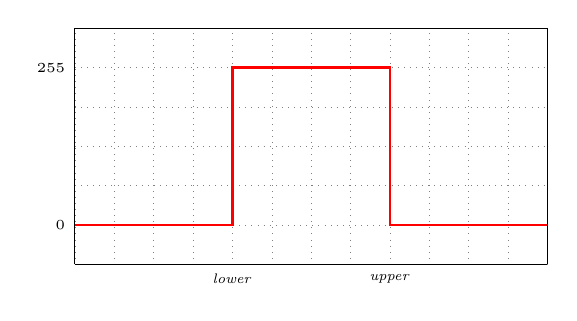
\begin{tikzpicture}[xscale=1.0,yscale=1.0]
\draw [help lines,dotted,step=.5] (0,0) grid (6,3);
\draw [thin] (0,0) -- (0,3);
\draw [thin] (0,3) -- (6,3);
\draw [thin] (0,0) -- (6,0);
\draw [thin] (6,0) -- (6,3);
\node [below] at (2,0) {\tiny\textit{lower}};
\node [below] at (4,0) {\tiny\textit{upper}};
\node [left] at (0,2.5) {\tiny $255$};
\node [left] at (0,0.5) {\tiny\ $0$};
\draw [thick,red] (0,0.5) -- (2,0.5) -- (2,2.5) -- (4,2.5) -- (4,0.5) -- (6,0.5);
\end{tikzpicture} 
\caption{Binary thresholding function.}
\label{fig:BinaryThresholdFunc}
\end{figure}

\subsubsection{Initial Contours Generation}

The initial contours will be generated using the fast marching method \cite{Sethian1999}, a numerical method used for the tracking of the propagating interface.
The evolution begins from the appropriately selected seeding points.
For the planar curve $\mathcal{C} = \{(x,y) | T(x,y) = t\}$,
%\begin{equation}
%\label{eqn:Curves}
%\mathcal{C}(t) = \{(x,y) | T(x,y) = t\},
%\end{equation}
where $(x,y)$ represents some point in the image, and $T(x,y)$ marks the time when the interface crosses the point.
The algorithm realizes the tracking of the evolution by solving the following equation
\begin{equation}
\label{eqn:Eikonal}
1 = | \nabla T | F,
\end{equation}
where $F$ denotes the speed in the normal direction at some point $(x,y)$.
The interface propagates inwards when $F < 0$; and propagates outwards when $F > 0$.
If the speed function $F$ only depends the position of the point, then (\ref{eqn:Eikonal}) reduces to the Eikonal equation.
The resultant images are the time-crossing map in which the time-of-arrival at every point are computed.

\subsection{Geodesic ``Snakes" Evolution}

The geodesic ``snakes" method \cite{Caselles1997}, based on the classical ``snakes" model \cite{Kass1988}, is aimed to implement the detection of the boundaries of multiple objects simultaneously without additional routines. %
The idea of the classical model is to evolve a contour $\mathcal{C}$ such that the edge of the object can be detected, where the contour cannot deal with the change of its topology so that detecting more than one object in the image is impossible \cite{Caselles1997}. %.
Computationally, the adopted geodesic ``snakes" connects the geodesic calculation and the level set evolution.

The goal of this method is to find the following minimum:
\begin{equation}
\label{eqn:MinModel}
\min \int_0^1 g(|\nabla I_{\sigma} ( \mathcal{C} (q) )|) |\mathcal{C}' (q)| dq,
\end{equation}
% Thus the problem has been shifted from the minimization of (\ref{eqn:ParticularSnakes}) to the geodesic computation.
where $\mathcal{C}(q):[0,1]\rightarrow \mathrm{R}^2$ denotes the parametrized planar curve, $I_{\sigma}:[0,a]\times [0,b]\rightarrow \mathrm{R}^{+}$ represents the input image, $g(\cdot): [0, \infty) \rightarrow \mathrm{R}^{+}$ is a monotonically decreasing function. %
In (\ref{eqn:MinModel}), $g(\cdot)$ is equivalent to the speed of the evolution of the curve.
And it is also dependent upon the geometry of the image content.
For the ideal edges of the objects to be detected, the choice of parameter $g(\cdot)$ is independent of their geodesic computation.

To find the minimum of (\ref{eqn:MinModel}), the geodesic flow is calculated by
\begin{equation}
\label{eqn:EvolutionModel}
\mathcal{C}_t = \frac{\partial \mathcal{C}}{\partial t} = g(I_{\sigma}) \kappa \mathcal{N} - (\nabla g(I_{\sigma}) \cdot \mathcal{N}) \mathcal{N},
\end{equation}
where $\kappa$ is the Euclidean curvature of $\mathcal{C}$, $\mathcal{N}$ is the unit inward normal vector. %, and the right-hand side of the equation is the computation of Euler-Lagrange.
Equation (\ref{eqn:EvolutionModel}) shows the way $\mathcal{C}$ propagating towards the edges of the targets, i.e., the initial curve $\mathcal{C}(0)$ evolves to a (local) minimum of (\ref{eqn:MinModel}).

According to (\ref{eqn:EvolutionModel}), this evolution will stop at edges of the targets when $\mathcal{C}_t = 0$.
%According to (\ref{eqn:EvolutionModel}), this evolution will stop when $\frac{\partial \mathcal{C}(t)}{\partial t} = 0$, meaning that the boundaries of the objects are detected.
Imagine that $\mathcal{C}$ is a level-set of a function $u(\cdot):[0,a] \times [0,b] \rightarrow \mathrm{R}$, and considering (\ref{eqn:MinModel}), the former evolution (\ref{eqn:EvolutionModel}) is transformed to finding the steady state solution of the following equation: %
\begin{equation}
\label{eqn:LevelSetModel}
u_t = \frac{\partial u}{\partial t} & = g(I_{\sigma}) |\nabla u| \kappa + \nabla g(I_{\sigma}) \cdot \nabla u,
%\begin{split}
%\frac{\partial u}{\partial t} & = |\nabla u| \textrm{div} \left(g(I_{\sigma}) \frac{\nabla u}{|\nabla u|}\right) \\
%                              %& = g(I_{\sigma}) |\nabla u| \textrm{div} \left(\frac{\nabla u}{|\nabla u|}\right) + \nabla g(I_{\sigma}) \cdot \nabla u \\
%                              & = g(I_{\sigma}) |\nabla u| \kappa + \nabla g(I_{\sigma}) \cdot \nabla u,
%\end{split}
\end{equation}
where $\kappa = \textrm{div}\left( \nabla u \cdot |\nabla u|^{-1} \right)$.
%where $\kappa = \textrm{div}\left(\frac{\nabla u}{|\nabla u|}\right)$.

To increase the ``attraction" to the contour towards the edges, a term is added to (\ref{eqn:LevelSetModel}):
\begin{equation}
\label{eqn:GeodesicDriver}
%\label{eqn:Geodesic1}
u_t = g( I_{\sigma} )( c + \kappa ) |\nabla u| + \nabla u \cdot \nabla g(I_{\sigma}),
%u_t = |\nabla u| \textrm{div} \left(g(I_{\sigma}) \frac{\nabla u}{|\nabla u|}\right) + c g(I_{\sigma}) |\nabla u|,
\end{equation}
where $c$ is a constant and $c \in \mathrm{R}^+$.
Regarding (\ref{eqn:LevelSetModel}), %the above equation can be rewritten as
%\begin{equation}
%\label{eqn:Geodesic2}
%u_t = g( I_{\sigma} )( c + \kappa ) |\nabla u| + \nabla u \cdot \nabla g(I_{\sigma}).
%\end{equation}
% which means that the level sets move according to
equation (\ref{eqn:GeodesicDriver}) can be transformed to the following evolution equation
\begin{equation}
\label{eqn:GeodesicEvolution}
\mathcal{C}_t = g(I_{\sigma}) ( c + \kappa ) \mathcal{N} - ( \nabla g(I_{\sigma}) \cdot \mathcal{N} ) \mathcal{N}.
\end{equation}
The solution to this problem is equivalent to the zero level-set of the steady state (i.e., $u_t = 0$) of (\ref{eqn:GeodesicDriver}).

%\subsection{Iso-Surface Extraction}
%
%To visualize the surface model, the surface information should be firstly extracted by the marching cubes method \cite{Lorensen1987MC}.
%As the initial step of surface extraction, arrays of cubes are created from the input with each cube consisting of eight pixels (four from one slice and the other four from the next slice).
%Then the index for each cube is calculated by comparing the eight intensity values to the specified isovalue corresponding to the surfaces of the objects.
%By referring to the triangulated cases with the indexes, the intersection patterns of the objects and the cubes can be roughly determined.
%Then the precise edge intersections are computed using linear interpolation with the intensity values at each vertex of the cubes.
%After that, the unit normals to the surface at each vertex of these cubes are computed via central differences.
%The resulting triangles are then sent to the graphics systems and displayed by standard rendering techniques.
% The isovalue representing the edge of the segmented target is selected.
% Then the 3-D model of the target can be reconstructed.
% That is the 3-D surface model of the lumen of the aorta. 